% \documentclass[12pt]{mitthesis}
% \usepackage[pdftex]{graphicx}
% \usepackage{kylesthesis}
% \begin{document}
% \tableofcontents
% \clearpage

\chapter{Introduction}
\label{chapter:intro}

\section{Objectives}

Intramolecular decay processes in electronically excited organic
molecules are dominated by the structure of triplet states
\cite{mcglynn69, medvedev95}.  Molecules in triplet states are
long-lived (metastable); optical transitions to the ground state
violate the selection rule $\Delta S = 0$.  Because triplet states are
optically inaccessible from the ground state, they are a difficult
target for spectroscopists.  From a chemical standpoint, molecules in
triplet states are energy carriers.  The long lifetimes ($\tau > 30$
\microsec) and chemically significant internal energies ($E_T >
30,000$ \rcm) of triplet molecules make them important chemical
reaction intermediates \cite{calvert66}.

Intersystem Crossing (ISC) is the dynamical manifestation of mixing
between singlet and triplet excited states \cite{robinson67,
  kommandeur87, lombardi88, tramer05}.  ISC is understood primarily as
a statistical process, where an electronically excited state decays
into a bath of undistinguished triplet states.  The general behavior
of ISC is categorized by the product of the average singlet-triplet
matrix element, $\langle H_{sm} \rangle$, and the local density of
triplet states, $\rho_m$ \cite{robinson67, kommandeur87, freed76}.
When $\langle H_{sm} \rangle \rho_m \ll 1$, the system is said to be
in the ``small-molecule limit.''  In the small molecule limit,
singlet$\sim$triplet mixing may often be treated as a two-level
problem, and the properties of the individual singlet and triplet
levels may be determined by deperturbation.  When $\langle H_{sm}
\rangle \rho_m \gg 1$, the system approaches the ``large molecule
limit.''  In this case, the density of triplet states is so large that
the natural width of singlet-mixed eigenstates exceeds the average
energy spacing.  The problem of singlet$\sim$triplet mixing is treated
in a statistical manner, based on the average properties of the
triplet levels.  When $\langle H_{sm} \rangle \rho_m \approx 1$, the
system is in the ``intermediate case,'' characterized by mixing
between a singlet level and a number of discrete triplet levels.

For many molecules, the dynamics of intersystem crossing cannot be
classified simply by one of the schemes above.  A more general
``tier'' model is proposed to understand the dynamics of systems where
some of the mixing occurs indirectly in the zero-order picture
\cite{stuchebrukhov93a, stuchebrukhov93b}.  Such a situation is found
in the acetylene molecule, where vibrational levels of the $T_3$
electronic state mediate mixing between the first excited singlet
state, $S_1$, and the remaining triplet states, $T_{1,2}$.  At
energies below the first dissociation limit, the product $\langle
H_{S_1 T_3} \rangle \rho_{T_3}$ is much less than 1.  Thus, $S_1 \sim
T_3$ mixing is categorized in the small molecule limit.  Conversely,
the product $\langle H_{T_3 T_{1,2}} \rangle \rho_{T_{1,2}}$ is on the
order of 1.  Mixing between the first and second tiers is categorized
in the intermediate case.

In the limit of small $T_3$ level density, the tier model simplifies
to a ``doorway-mediated'' model.  In most cases, one vibrational level
of $T_3$, called the doorway state, dominates the $S_1 \sim T_3$
mixing.  In this thesis, the doorway model for intersystem crossing is
examined and characterized for cases where a doorway state is
non-degenerate with a perturbed singlet level.

\section{Spectroscopic investigations of acetylene triplet states}

The first experimental detection of acetylene in the triplet state was
reported by Burton and Hunziker in 1972 \cite{burton72}.  They
produced triplet acetylene molecules by the process of mercury
photosensitization.  Mercury photosensitization is the electronic
excitation of molecules in collisions with excited mercury atoms.  The
excited atoms are produced by absorption of 254 nm radiation from a
mercury resonance lamp.  The process has been known to photochemists
since the 1920's \cite{calvert66, cairo22}.  Triplet acetylene was
detected in the experiments by collisional excitation of biacetyl,
which emits phosphorescence in the visible region of the spectrum
\cite{burton72}.  The energy of triplet acetylene was estimated to be
roughly 2.6-4.7 eV.

Subsequent experiments investigated the geometry of triplet acetylene.
The spectrum of a triplet-triplet transition in the near
infrared was observed by Wendt and coworkers \cite{wendt79}.  Triplet
acetylene was again produced by a method of mercury
photosensitization.  The spectrum was assigned to the only allowed
triplet-triplet transition among the low-lying electronic states of
acetylene, $\tilde{d} \; ^3A_2 \leftarrow \tilde{a} \; ^3B_2$.  This
confirmed the existence of the predicted lowest energy triplet state,
\emph{cis}-bent $\tilde{a}$ $^3B_2$.  Subsequently, Lisy and Klemperer
used a low-energy electron gun to produce metastable acetylene
molecules in an effusive beam, which they detected via electron
ejection from a cesium surface located 80 cm downstream \cite{lisy80,
  hemminger76}.  They measured a negligible electric dipole moment for
the lowest energy metastable triplet state, consistent with a
\emph{trans}-bent structure at approximately 4.7 eV.

The relative energies of the observed \emph{cis} and \emph{trans}
triplet states were the subject of some debate, due to the two
apparently conflicting observations.  The apparent disparities are
explained by the fact that spin-orbit perturbations high vibrational
levels of the ground state are electronically allowed for the
\emph{cis}-bent state, but only vibronically allowed for the
\emph{trans}-bent state \cite{lundberg93}.  Since the \emph{cis}-bent
triplet is more efficiently mixed with high vibrational levels of the
ground state, it is less efficiently detected via electron emission
from a metal surface.  The observation of Lisy and Klemperer is
therefore consistent with the \emph{ab initio} determination that the
lowest triplet state of acetylene is \emph{cis}-bent
\cite{lundberg93}.

Electron Energy Loss Spectroscopy (EELS) has provided some more recent
low-resolution information on the linear triplet structures
\cite{dressler87, swiderek97}.  Assignments of the \emph{cis} and
\emph{trans}-bent triplet states in condensed phase EELS of acetylene
is in general agreement with the theory, which we review in the next
section \cite{malsch98}.


\section{Survey of the low-lying triplet electronic states of
  acetylene: \emph{ab initio} calculations}

% \POINT{Summarize the electronic structure of the acetylene valence
%   triplet states.  Show molecular orbitals and energy level diagrams.}
% \POINT{Discuss the change in geometry, cis and trans wells.}

The valence electronic states of acetylene result from the promotion
of one electron from a bonding $\pi$ orbital to an antibonding $\pi^*$
orbital.  Figure \ref{fig:mol-orbitals} shows the principal molecular
orbital configurations for the four lowest energy excited electronic
states of acetylene \cite{yamaguchi93}.  The in-plane antibonding
orbital, $\pi^*(a_g)$, is stabilized by a change in \ce{CCH} bond
angle, while the out-of-plane antibonding orbital is not
\cite{walsh53, demoulin75, wetmore78}.  Balanced against the
destabilization of fully filled $\sigma$-bonding orbitals, this effect
gives rise to potential energy minima in \emph{cis}-bent and
\emph{trans}-bent geometries for the low-lying electronic states of
acetylene, $S_1$, $T_1$, $T_2$, and $T_3$.

\begin{figure}
  \caption{Principal molecular orbital configurations for the four
    lowest energy \emph{trans}-bent excited states of acetylene
    \cite{yamaguchi93}.  The vertical position of an orbital in the
    diagram does not accurately reflect its total energy:
    stabilization of the $\pi^*(a_g)$ antibonding orbital in
    \emph{trans}-bent geometries is much larger than the
    de-stabilization of the $\pi(a_u)$ bonding orbital
    \cite{wetmore78}.  The four electronic states, $T_1$, $T_2$,
    $T_3$, and $S_1$, are listed in order of increasing energy
    ($T_e$).  For simplicity, the fully filled orbitals,
    $(1\sigma_g)^2 (1\sigma_u)^2 (2\sigma_g)^2 (2\sigma_u)^2
    (3\sigma_g)^2$, are not shown.  The $S_1$ and $T_3$ electronic
    states differ by one antibonding spin orbital.}
  \label{fig:mol-orbitals}
  \centering
  \vspace{1cm}
  \setlength{\unitlength}{1cm}
  \begin{picture}(8,8)
    \put(-0.5,1){$\pi\:(b_u)$}
    \put(-0.5,2){$\pi\:(a_u)$}
    \put(-0.5,4){$\pi^*(a_g)$}
    \put(-0.5,5){$\pi^*(b_g)$}


    \put(1,1){\line(1,0){1}}
    \put(1,2){\line(1,0){1}}
    \put(1,4){\line(1,0){1}}
    \put(1,5){\line(1,0){1}}
    \put(1.25,0.85){\Large{$\upharpoonleft$}}
    \put(1.25,1.85){\Large{$\upharpoonleft$}}
    \put(1.5,1.85){\Large{$\downharpoonright$}}
    \put(1.5,3.85){\Large{$\upharpoonright$}}
    \put(1.333,7){$T_1$}
    \put(1.333,6){$B_u$}

    \put(3,1){\line(1,0){1}}
    \put(3,2){\line(1,0){1}}
    \put(3,4){\line(1,0){1}}
    \put(3,5){\line(1,0){1}}
    \put(3.25,0.85){\Large{$\upharpoonleft$}}
    \put(3.25,1.85){\Large{$\upharpoonleft$}}
    \put(3.5,0.85){\Large{$\downharpoonright$}}
    \put(3.5,3.85){\Large{$\upharpoonright$}}
    \put(3.333,7){$T_2$}
    \put(3.333,6){$A_u$}


    \put(5,1){\line(1,0){1}}
    \put(5,2){\line(1,0){1}}
    \put(5,4){\line(1,0){1}}
    \put(5,5){\line(1,0){1}}
    \put(5.25,0.85){\Large{$\upharpoonleft$}}
    \put(5.25,1.85){\Large{$\upharpoonleft$}}
    \put(5.5,0.85){\Large{$\downharpoonright$}}
    \put(5.5,4.85){\Large{$\upharpoonright$}}
    \put(5.333,7){$T_3$}
    \put(5.333,6){$B_u$}


    \put(7,1){\line(1,0){1}}
    \put(7,2){\line(1,0){1}}
    \put(7,4){\line(1,0){1}}
    \put(7,5){\line(1,0){1}}
    \put(7.25,0.85){\Large{$\upharpoonleft$}}
    \put(7.25,1.85){\Large{$\upharpoonleft$}}
    \put(7.5,0.85){\Large{$\downharpoonright$}}
    \put(7.5,3.85){\Large{$\downharpoonright$}}
    \put(7.333,7){$S_1$}
    \put(7.333,6){$A_u$}

  \end{picture}
  \vspace{2cm}
\end{figure}

% \POINT{Discuss the forbiddenness of the singlet transition and how it
%   is made allowed only in the \emph{trans} well.}
The $\tilde{A}^1A_u \leftarrow \tilde{X}^1\Sigma_g$ electronic
transition is localized in the \emph{trans} well of acetylene, and the
process of intersystem crossing between singlet and triplet excited
states proceeds locally in this geometry.  For this reason, we no
longer explicitly write the geometry when referring to the valence
electronic states of acetylene; a \emph{trans}-bent geometry is
implied unless otherwise stated.  The normal modes of $S_1$
($\tilde{A}\;^1A_u$) acetylene are summarized in Figure
\ref{fig:modes}, for reference.

\begin{figure}
  \centering
  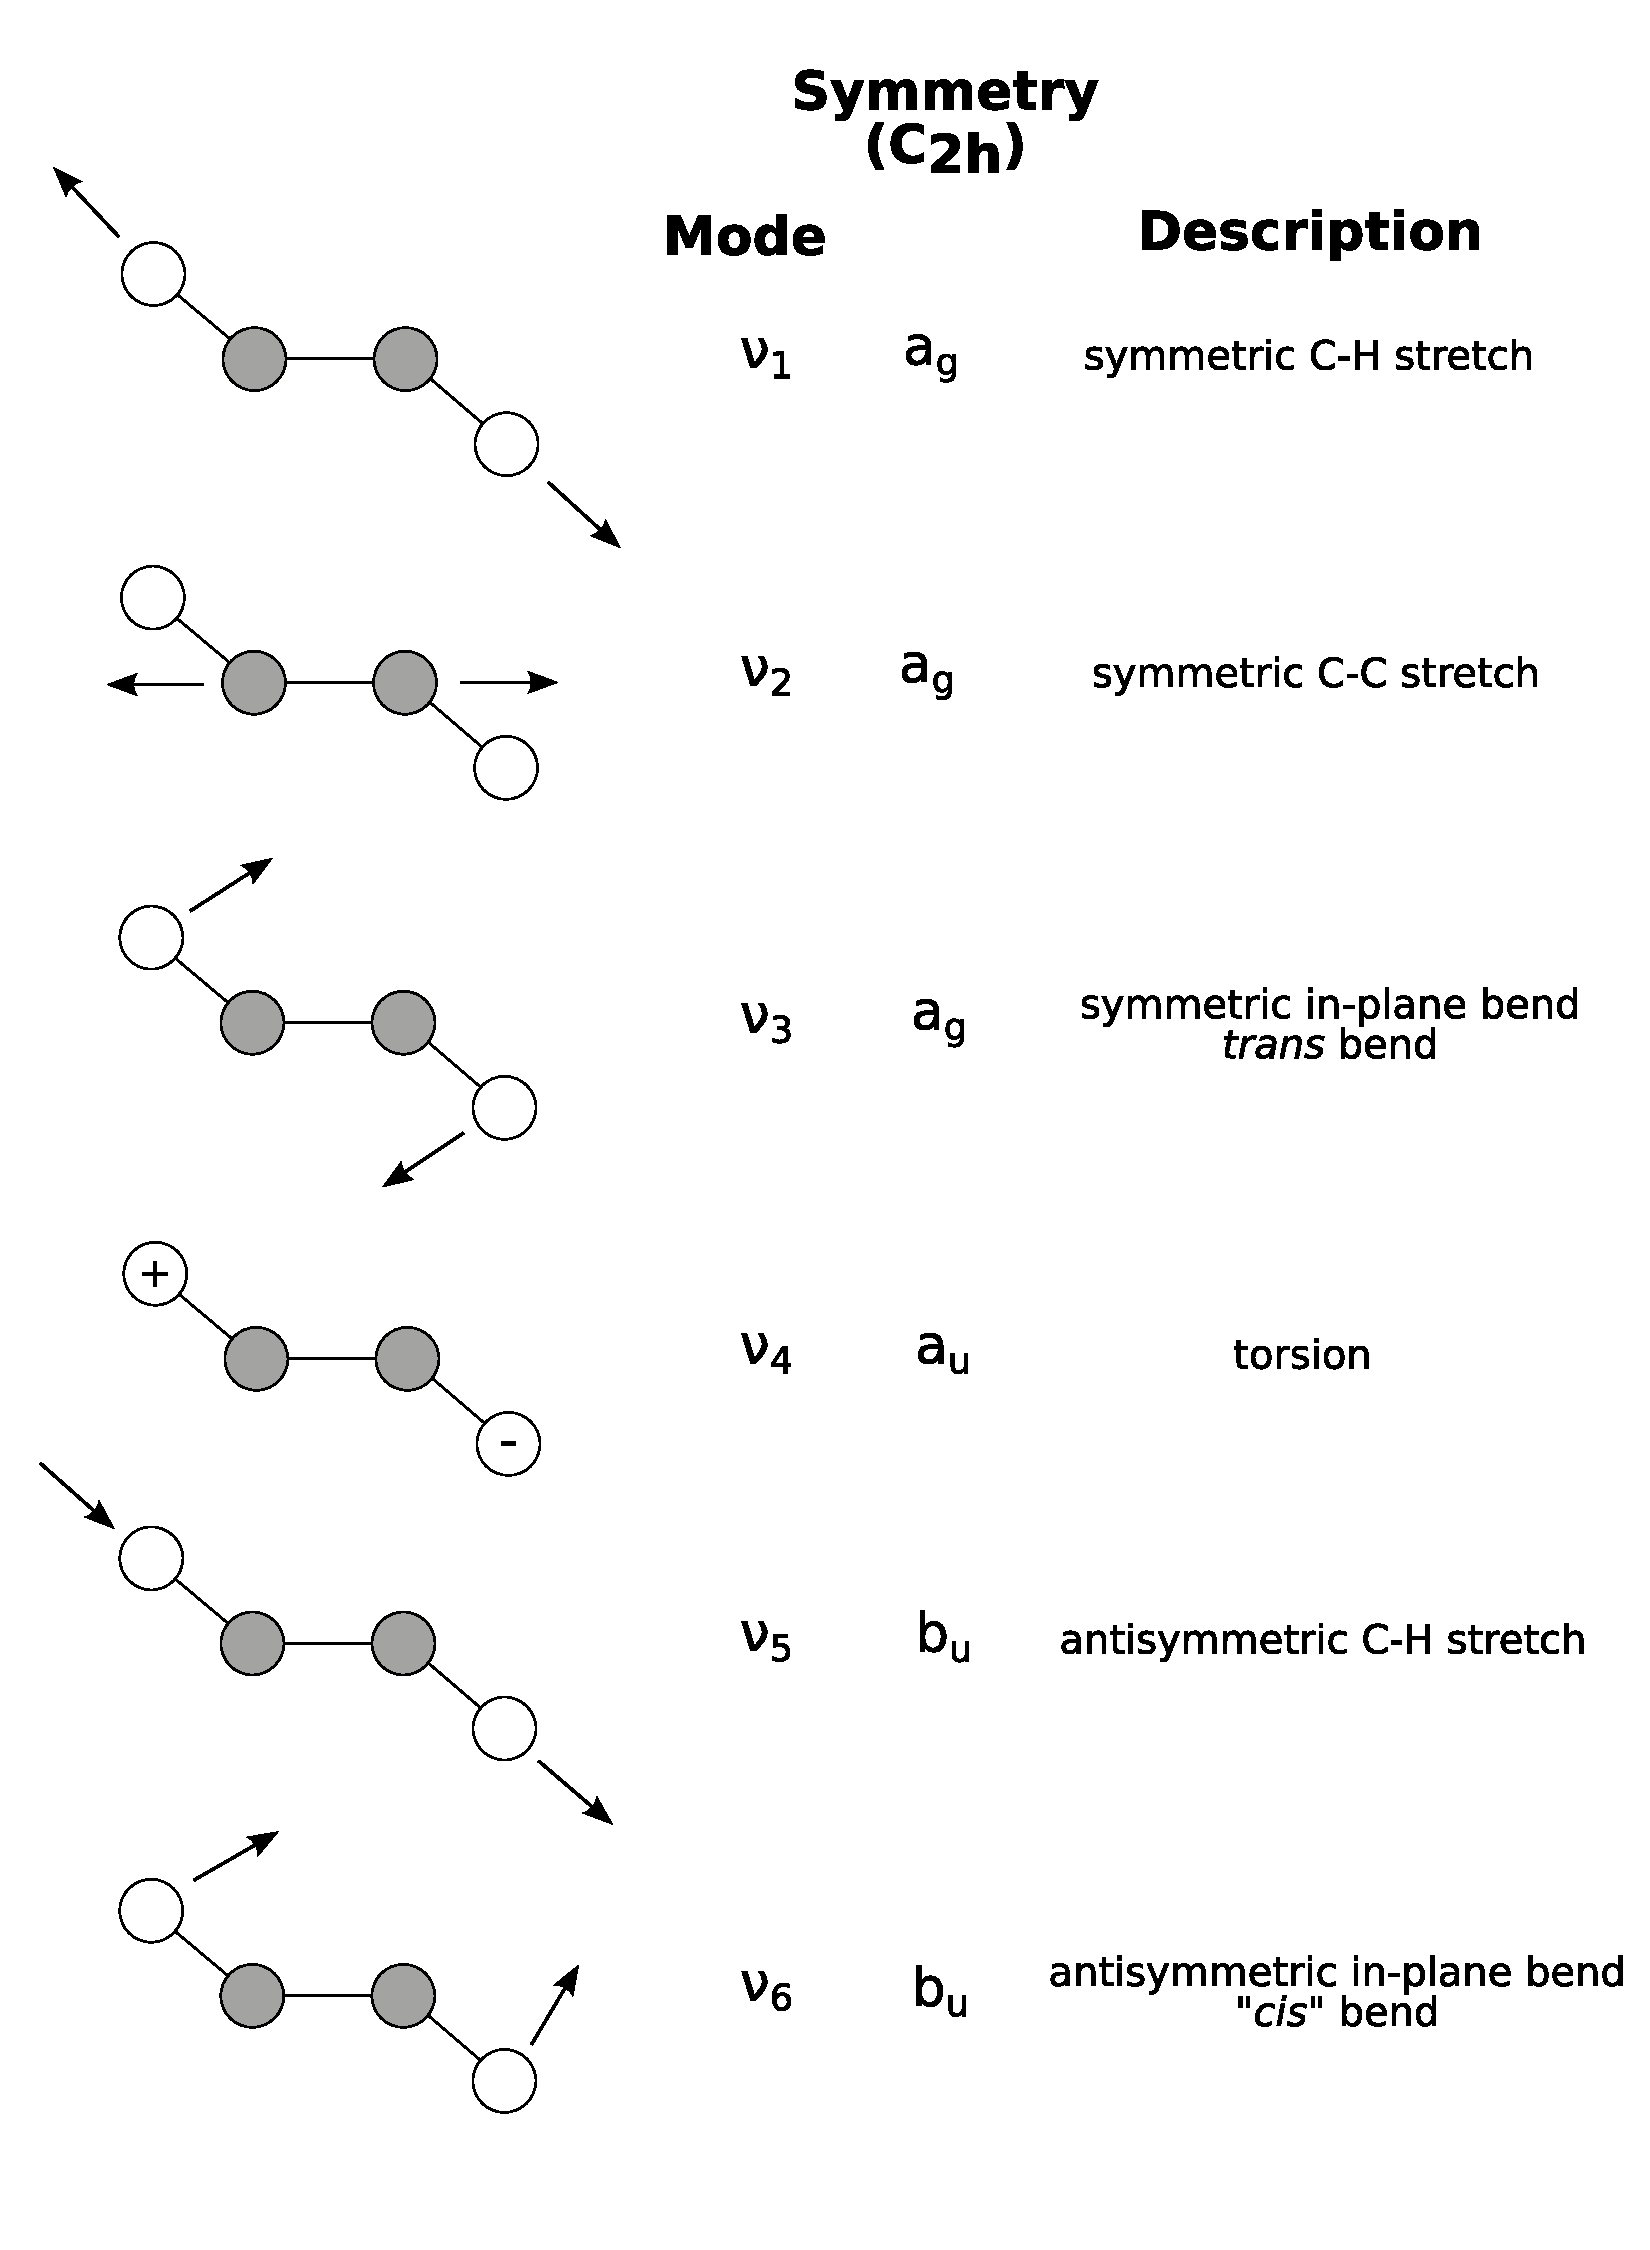
\includegraphics[width=5.8in]{s1-modes.pdf}
  \caption{Summary of normal modes for planar, \emph{trans}-bent $S_1$
    ($\tilde{A}^1A_u$) acetylene.  The bending modes, $\nu_3$,
    $\nu_4$, and $\nu_6$, are of particular interest for their role in
    $S_1 \sim T_3$ mixing.}
  \label{fig:modes}
\end{figure} 

% \POINT{Discuss spin-orbit coupling with S1 state.  Show the spin-orbit
%   operator and one-electron matrix elements among the triplet states.
%   The $\ell_+s_-$ operator requires a change in spin-orbital.
%   (Examples of Slater determinants: p.59 of 11/2007--1/2008 notebook
%   [\ce{CO2}])}

% \POINT{Many ab initio studies of acetylene triplet states
%   \cite{demoulin75, lischka86, cui96, cui97, malsch98, dallos02,
%     ventura03, thom07}.  Give a summary of the most recent theoretical
%   results.}  

Potential surfaces for the $T_1$ and $T_2$ states of acetylene have
been computed in many \emph{ab initio} studies \cite{demoulin75,
  wetmore78, lischka86, yamaguchi93, cui96, cui97, malsch98, dallos02,
  ventura03}.  The $T_1$ and $T_2$ states have planar,
\emph{trans}-bent equilibrium geometries, similar to $S_1$
\cite{demoulin75, wetmore78, yamaguchi93}.  The minimum of the $S_1$
electronic surface is above the $T_1$ and $T_2$ isomerization barriers
\cite{vacek96, sherrill96}.

The equilibrium geometry of $T_3$ is near-linear, \emph{trans}-bent,
and twisted approximately 75\degrees\ out of plane along the torsional
coordinate \cite{ventura03, thom07}.  The electronic energy of $T_3$
has been determined in several \emph{ab initio} calculations
\cite{malsch98, ventura03, thom07}.
% Malsch and
% coworkers found an energy of 5.46 eV, almost 2200 \rcm\ higher than
% their calculated energy for $S_1$ \cite{malsch98}.  
The most recent calculation of the $T_3$ electronic surface, carried
out by Bryan Wong and coworkers, determined an energy separation
$T_e(S_1)-T_e(T_3)$ of only 270 \rcm\ \cite{thom07}.
%  which places the $T_3$ state at
% approximately the same energy as the $S_1$ state \cite{thom07}.  It is
% in light of these most recent calculations that we continue our
% discussion.

% \POINT{Almost no direct experimental evidence concerning triplet
%   states.  No spectra for trans-bent triplet states, although spectra
%   have been recorded for the cis-well.}

% \POINT{Discuss propensity/selection rules for triplet-triplet
%   transitions.  No allowed T-T electronic transitions among the
%   valence states in the trans well.}

% \POINT{Discuss density of triplet vibrational levels as a function of
%   energy.  Discussion of Ryan and Bryan's paper here \cite{thom07}?}

% \POINT{Show the vibrational modes of \emph{trans} acetylene and their
%   symmetries.  Explain selection rules for transitions from the ground
%   state.  (See p.33 of1/2007--3/2007 notebook.)}


\section{A hierarchy of electronic coupling in acetylene: evidence from
  Zeeman anticrossing experiments}

A series of Zeeman Anticrossing (ZAC) experiments, carried out by
Dupr\'{e} and coworkers, established a heirarchy of
singlet$\sim$triplet mixing in acetylene \cite{dupre91, dupre93,
  dupre95a, dupre95b}.  The mixing is controlled by the relative
magnitudes of matrix elements between electronic states.  The
conclusions of the Dupr\'{e} ZAC experiments are of fundamental
importance to the work in this thesis.  We summarize the experiments
in some detail.

In a Zeeman anticrossing experiment, the excitation laser is fixed on
an optical transition terminating in a nominally singlet rovibronic
level of the molecule, and a magnetic field is tuned.  As the magnetic
field is increased, the energies of triplet-mixed levels tune through
resonance with the singlet.  Relative to the singlet level at $E=0$,
the energy of a mixed triplet level is (by the linear Zeeman effect)
\begin{equation}
  E = g \, M_s \, \mu_B \, (B-B_0),
\end{equation}
where $g$ is the $g$-factor of the mixed-triplet level, $M_s$ is the
lab-fixed projection of spin, $B_0$ is the field required to bring the
level to resonance with the singlet, and $\mu_B$ is the Bohr magneton
\cite{lombardi88}.  An excited electron that is not coupled to the
molecular axis (Hund's case ($b$) limit) has a $g$-factor of $2.0023$.
When the singlet level and one of the weakly interacting background
levels are tuned to exactly the same energy by the magnetic field,
they become 50:50 mixed.  Under these circumstances, half the
molecules excited in the experiment decay by collision instead of
fluorescence, and the fluorescence intensity decreases by 50\%.  The
\emph{width} of the resonance is proportional to the matrix element
between the bright state and the interacting level:
\begin{equation}
  \Delta B = \frac{4\,V}{g\,\mu_B}.
\end{equation}

Dupr\'{e} and coworkers measured the $0-8$ T anticrossing spectra of
the $J'=0$, $K'=0$ rovibronic levels in $S_1$ $\nu_3'=0-3$
\cite{dupre91}.  The density of mixed-triplet levels was observed to
increase rapidly with excitation in $\nu_3$.  Because density of
states is larger than the number of $T_{1,2}$ levels, they concluded
that the triplet levels must mix with and contaminate the denser
manifold of $S_0$ levels.  However, increased $T_{1,2} \sim S_0$
coupling does not by itself make more mixed-triplet levels accessible
to cross with the $S_1$ level.  The $S_1$ level can only undergo
triplet-mediated mixing with $S_0$ levels over an energy range on the
order of the $S_1 \sim T$ matrix element.  Therefore, they concluded
that coupling between $S_1$ and a subset of the triplet levels $T$
must increase to make the dense manifold of mixed $T_{1,2} \sim S_0$
levels observable in the experiment.

A rapid increase in anticrossing linewidth with excitation in $\nu_3$
was observed in the same study \cite{dupre91}.  Since the linewidth is
proportional to the $S_1 \sim T$ matrix element, this supports the
conclusion that the $S_1 \sim T$ coupling is increasing with
excitation in $\nu_3$.  Accounting for both observations, the authors
are able to exclude several possible mechanisms for the increase in
anticrossing density.  Direct $S_1 \sim S_0$ internal conversion is
ruled out because there is nothing to account for a sudden increase
in $S_1 \sim S_0$ vibrational overlap integrals.  The possibility that
the $S_0$ dissociation limit may increase the total density of states
is ruled out because any increase in state density would be
accompanied by a decrease in vibrational overlap integrals.

Dupr\'{e} and Green characterized a wide anticrossing in the $3\nu_3'$
$J'=0$ $K'=0$ level, attributed to a triplet level with relative
energy $\Delta E = \pm 6.67$ cm$^{-1}$ \cite{dupre93}.  Thom and
coworkers provide a useful summary of this experiment in their recent
article \cite{thom07}.  Many weak anticrossings with nominal $S_0$
levels can be seen perturbing the strong $S_1 \sim T$ anticrossing.
The zero-field matrix element is $0.29$ cm$^{-1}$ if $K_{T}=0$, or
$0.58$ if $K_{T}=1$ \cite{thom07}.

In further studies, Dupr\'{e} and coworkers undertook the individual
analysis of approximately 60 anticrossings from the $\nu_3'=0-2$
spectra \cite{dupre95a}.  The analysis reveals a large variation in
measured $g$ factors, which implies that the $T_{1,2}$ levels are
highly mixed.  Mixing between triplet states, according to the
selection rule $\Delta M_S = \pm 1$, causes the $g$ factors to vary
from the expected value of $2$.  Strong $S_0 \sim T_{1,2}$ mixing is
ruled out because it would cause the $g$ factors to be close to zero.
The authors also observed that all quantum beat frequencies vary as a
function of field strength \cite{dupre95a}.  Direct mixing (``internal
conversion'') between $S_1$ and $S_0$ is therefore ruled out, since
it would cause the frequencies of quantum beats to be approximately
constant as a function of magnetic field strength ($M_S=0$ for all
singlet levels).

In the final paper of the series, Dupr\'{e} derives the product
$\rho_{vib} \cdot \langle V \rangle$ from the Fourier transform of
anticrossing spectra for $\nu_3=0-4$ \cite{dupre95b}.  He determines
that the product $\rho_{vib} \cdot \langle V \rangle$ increases
exponentially from $0\nu_3$ to $4\nu_3$.  The density of states does
not increase appreciably over this energy range, so the effect must
arise from an increasing matrix element.

The authors proposed an order of interaction strengths: $T_1 \sim T_2
\gg S_1 \sim T \gg S_1 \sim T_{1,2} \gg S_0 \sim T_{1,2} \gg S_1 \sim
S_0$\footnote{The authors do not explicitly state the inequality $S_1
  \sim T \gg S_1 \sim T_{1,2}$, but it is implied by the rapid
  increase in anticrossing density with excitation in $\nu_3'$.}
\cite{dupre95b} The first inequality is supported by the large
variation in measured $g$ factors \cite{dupre95a}.  The inequality
$S_1 \sim T_{1,2} \gg S_0 \sim T_{1,2}$ allows for the large number of
$S_0$ levels detected in the ZAC experiments \cite{dupre91}.  The
third inequality, $S_0 \sim T_{1,2} \gg S_1 \sim S_0$, states that the
internal conversion process from $S_1$ to $S_0$ is triplet-mediated,
as supported by the variation in quantum beat frequencies with
magnetic field \cite{dupre95a}.

Two mechanisms are put forward to explain the rapid increase in
anticrossing density with excitation in $\nu_3'$: an $S_1 \sim T_3$
curve crossing and a $T_2$ linear isomerization barrier \cite{dupre91,
  dupre95b}.  Under the first mechanism, the observed $S_1 \sim T$
coupling is induced by a sparse manifold of $T_3$ levels, most of
which are located outside the tuning range of the magnetic field.
Under the second proposed mechanism, the $T_2$ linear isomerization
barrier causes the vibrational overlap between $T_2$ levels in the
\emph{cis}-well and $S_1$ levels in the \emph{trans}-well to increase
in the region of the linear turning point.  Although the second
mechanism is energetically possible, subsequent \emph{ab initio}
calculations rule out the linear $T_2$ barrier in favor of the first
mechanism \cite{vacek96, sherrill96, cui96, cui97, ventura03}.

% The main conclusions are summarized as follows.
% \begin{inparaenum}
% \item Mixing between $T_{1}$ and $T_2$ dominates the intramolecular
%   dynamics in the energy region of the study, evidenced by widely
%   varying local Land\'{e} g-factors ($0.3-2.0$).
% \item The $T_1 \sim T_2$ coupling strength increases only slightly
%   over the energy range of $0\nu_3'-2\nu_3'$.  This is evidenced by an
%   observed decrease in the average Land\'{e} g-factor with energy.
% \item Mixing between the $S_1$ and $S_0$ electronic states is not the
%   result of direct internal conversion, but is induced by the mixed
%   $T_{1,2}$ levels.
% \item There is a rapid increase in $S_1 \sim T_{1,2}$ mixing in the
%   range of $0\nu_3'-2\nu_3'$, mediated by a special class of triplet
%   levels, $T$.  Matrix elements between $T$ and $S_1$ mediate the $S_1
%   \sim T_{1,2}$ mixing.
% \end{inparaenum}
% These observations led the authors to propose a heirarchy of
% interactions between the electronic states of acetylene:
% \begin{equation}
%   T_1 \sim T_2 \gg S_1 \sim T \gg S_0 \sim T \gg S_1 \sim S_0
% \end{equation}



\section{$T_3$-mediated intersystem crossing in acetylene: evidence
  from laser-induced fluorescence and quantum beats}

The $T_3$-mediated doorway model of acetylene singlet$\sim$triplet
mixing is further supported by measurements of Laser-Induced
Fluorescence (LIF) and Zeeman quantum beats.  Ochi and coworkers
recorded LIF spectrum of the $3^2$ \Ka{1}, $3^3$ \Ka{1}, and $3^4$
\Ka{1} sublevels of $S_1$ acetylene, measuring fluorescence lifetimes
and the magnetic field dependence of quantum beats for each observed
line \cite{ochi91}.  They observe that the singlet-triplet mixing is
strongest for the $3^3$ \Ka{1} level, which is predicted to be
energetically proximal to a $S_1 \sim T_3$ surface crossing.

The 1994 study of Drabbels and coworkers is perhaps the only
experiment, aside from ZAC measurements, to record a fully resolved
spectrum of the $3^3$ \Ka{1} and $3^4$ \Ka{1} sublevels
\cite{drabbels94}.  They attribute the splittings in the spectrum to
direct $S_1 \sim T_{1,2}$ mixing, but this interpretation is
inconsistent with the profound changes in singlet-triplet mixing over
the 44,000$-$46,000 \rcm\ energy range.  Subsequent analysis has shown
that the Drabbels spectrum contains evidence for a local $S_1 \sim
T_3$ perturbation, which mediates the $S_1 \sim T_{1,2}$ mixing
\cite{altunata01}.

Recent investigations in our laboratory have led to the observation of
more triplet-perturbed levels in $S_1$ acetylene, as a fortunate side
effect in the deperturbation of the non-symmetric bending polyads
\cite{merer08, steeves08}.  Levels with excitation in the
non-symmetric bending modes are of particular interest because motion
along these coordinates may promote or reduce $S_1 \sim T_3$
vibrational overlap integrals.  Further information about the
non-symmetric bending modes, $\nu_4$ and $\nu_6$, would shed new light
on the nature of $S_1 \sim T_3 \sim T_{1,2}$ dynamics.

\section{Detection of laser-excited metastables by surface electron
  ejection}

The experimental technique of Surface Electron Ejection by
Laser-Excited Metastables (SEELEM) was developed by Ofer Sheh and Ori
Cheshnovsky to study intermediate-case ISC in organic molecules such
as aniline and isoquiniline \cite{sneh86, sneh88, sneh89a, sneh89b,
  sneh91}.  It is based on the well-established, more general
technique of metastable detection by electron ejection from surfaces
\cite{hotop96}.  The use of laser excitation to populate metastable
states in SEELEM is somewhat paradoxical because, by definition,
direct optical transitions to such states are strongly forbidden.  The
method of SEELEM detection sidesteps the problem of weak optical
transitions by maintaining a low level of background electron signal.

In essence, the SEELEM detector consists of a grounded metal surface
and an electron multiplier.  To eject an electron from the grounded
metal surface of the SEELEM detector, a molecule must possess a
vertical excitation energy in excess of the work function, $\Phi$, of
the metal.  A gold surface was used in most of the experiments
described in this thesis, $\Phi = 5.1$ eV.  Sneh and coworkers have
shown that excess vibrational energy in the molecule does not affect
the SEELEM sensitivity \cite{sneh86}.  The exception that proves the
rule is the \ce{NO} molecule, where vibrations in the excited state
have a drastic impact on the dipole moment\cite{white05}.

The SEELEM technique was applied to the study of smaller molecules by
Wodke and coworkers \cite{price92, drabbels95, morgan96, humphrey97}.
The SEELEM apparatus at MIT was designed and built by Kevin Cunningham
and Selen Altunata, first as a single-chamber experiment, and later as
a differentially-pumped, two-chamber experiment
\cite{cunningham-thesis, altunata-thesis}.  The apparatus was refined
by subsequent workers, such as Ryan Thom, who re-engineered the
mounting and electrical connections for the detector itself
\cite{thom-thesis}.

Previous acetylene SEELEM experiments have focused on the $3\nu_3'$
\Ka{1} sublevel of the $S_1$ electronic state.  Humphrey \emph{et.
  al.} observed an enhancement in SEELEM intensity for rotational
lines of $3\nu_3'$ \Ka{1} with $J' < 4$ \cite{humphrey97}.  They
attributed this effect to interference with a near-degenerate
vibrational sublevel of the $T_3$ electronic state.  The nature of
$S_1 \sim T_3$ interference effects in the SEELEM spectrum of this
sublevel was investigated further by Selen Altunata, who demonstrated
the relationship between the relative energy of the perturbing $T_3$
level and moments of the SEELEM intensity distribution
\cite{altunata00}.  Mishra and Thom provided new SEELEM assignments
and carried out a deperturbation of the perturbing triplet sublevel
using a reduced term value plot and an effective Hamiltonian fit
\cite{mishra04}.

A schematic diagram of the current LIF/SEELEM arrangement is shown in
Figure \ref{fig:apparatus}.  Laser radiation in the UV is provided by
the frequency doubled output of an Nd:YAG-pumped dye laser.  The laser
radiation enters the vacuum chamber (not shown), and crosses the path
of the molecular beam, indicated by a dashed line, approximately 2.5
cm downstream from a pulsed nozzle.  Fluorescence is gathered by $f$/4
optics at the point of laser excitation, passes through a UG-11
filter, and is collected by a photomultiplier tube (PMT).
Laser-excited metastable molecules travel through a 3 mm diameter
skimmer and into a second, differentially pumped vacuum chamber.
Approximately 34 cm from the point of laser excitation, the
metastables collide with the metal surface of the SEELEM detector.
Ejected electrons are collected by an electron multiplier that is
located immediately below the metal surface.

\begin{figure}
  \caption{Diagram of the LIF/SEELEM apparatus.  Laser radiation in
    the UV is provided by the frequency doubled output of an
    Nd:YAG-pumped dye laser.  The laser radiation enters the vacuum
    chamber (not shown), and crosses the path of the molecular beam,
    indicated by a dashed line, approximately 2.5 cm downstream from a
    pulsed nozzle.  Fluorescence is gathered by $f$/4 optics at the
    point of laser excitation, passes through a UG-11 filter, and is
    collected by a photomultiplier tube (PMT).  Laser-excited
    metastable molecules travel through a 3 mm diameter skimmer and
    into a second, differentially pumped vacuum chamber.
    Approximately 34 cm from the point of laser excitation, the
    metastables collide with the metal surface of the SEELEM detector,
    and ejected electrons are collected by an electron multiplier,
    located immediately below the metal surface.}
  \label{fig:apparatus}
  \centering
  
\includegraphics[width=7in,trim=1cm 0 0 0]{apparatus-bw}
\end{figure}

% We have reported transitions in SEELEM with signal levels as low as 1
% count per 2 laser pulses, 5 times the average rate of background
% SEELEM counts \cite{virgo07}.



\section{Summary}

%In this thesis, we develop new understanding of
%  new models, mechanisms, and methods of
% analysis to study 
% This thesis contributes to the general understanding of the process of
% doorway-mediated intersystem crossing.  

A doorway-mediated intersystem crossing model is well accepted for the
acetylene molecule.  However, its impact on the spectrum of most $S_1$
levels is poorly understood.  Triplet perturbations in the spectrum of
$S_1$ acetylene are ``seemingly random,''\footnote{A direct quote from
  a well-known spectroscopist, who shall remain nameless.} but the
doorway model insists emphatically that the perturbations are
\emph{not} random.  In this thesis, we establish and develop the
connection between the doorway model and spectroscopic measurements.
%Understanding a spectrum in terms of a doorway-mediated model 
This task requires new theory, new types of experiments, and new
methods of analysis.

% We show how the spectrum contains 
% With the experimental technique of SEELEM/LIF spectroscopy,
% we investigate singlet$\sim$triplet mixing in the acetylene molecule
% beyond the $\nu_3'=0-4$ levels.  In most cases, the $T_3$ vibrational
% levels responsible for mediating $S_1 \sim T_{1,2}$ mixing are not
% observed in the spectrum.  

In Chapter 2, we develop several frameworks for the problem of
doorway-mediated intersystem crossing.  Using these frameworks, the
relative statistical properties of LIF and SEELEM intensity
distributions are derived for several doorway-mediated model
Hamiltonians.  Of particular interest is the nature of interference
effects in each model Hamiltonian.

Moving beyond statistical properties, we demonstrate in Chapter 3 that
the parameters of a doorway-mediated model Hamiltonian are determined
by the frequencies and relative intensities of the absorption
spectrum.  The method of ``doorway deconvolution'' is presented as an
extension to the standard Lawrance-Knight-Lehmann deconvolution
technique.  The parameters of the model Hamiltonian are also derived
in terms of the statistical moments of the spectrum.

% Chapter 4 presents a new and extended analysis of the well-studied but
% incompletely characterized $3\nu'_3$ vibrational level of $S_1$
% acetylene, highlighting experimental evidence for a new model of
% doorway-mediated coupling.  The new model proposed for $3\nu'_3$
% includes two doorway states: one distant doorway state with a large
% matrix element controls the overall coupling strength, while another
% local doorway with a smaller matrix element is responsible for
% splittings at low values of the rotational quantum number $J$.

In Chapter 4, we report on new SEELEM/LIF spectra for a number of
$S_1$ vibrational levels. We discuss the ubiquitous role of $T_3$
vibrational levels as mediators of $S_1 \sim T_{1,2}$ mixing, and show
how the identity of a doorway level is imprinted on the spectrum.  A
theory of delayed fluorescence is developed and used as a primary tool
to understand the spectral patterns of doorway-mediated mixing.


% The complex interplay between bending vibrations
% and singlet$\sim$triplet mixing is apparent from the drastically
% different LIF/SEELEM spectra obtained.

The non-symmetric bending modes of $S_1$ acetylene, $\nu_4'$ and
$\nu_6'$, play an important role in the process of intersystem
crossing.  However, these two vibrations are normally mixed by strong
Darling-Dennison and $a$-type Coriolis resonances.  In Chapter 5, we
present the results of IR-UV double resonance SEELEM/LIF experiments,
where, by a careful choice of quantum numbers, the $\nu_4'$ and
$\nu_6'$ vibrations are unaffected by the two strong resonances.

In Chapter 6, we develop a new method for the production of metastable
molecules in a molecular beam.  The basis of this method is two-photon
optical pumping of metastable atoms, followed by electronic excitation
transfer in collisions.  The selection rules and transition
probabilities for two-photon excitation of the atoms are discussed for
mercury and xenon.  The method is applied to two chemical systems,
\ce{Xe}* + \ce{N2} and \ce{Hg}* + \ce{C2H2}.  


Chapter 7 concludes and summarizes the prospects for future research.

% \bibliography{master}
% \bibliographystyle{plain}
% \end{document}
% LocalWords:  Hunziker photosensitization photochemists nm biacetyl Hemminger
% LocalWords:  Wendt cis Lisy Klemperer vibronically detectivity Intramolecular
% LocalWords:  spectroscopists Intersystem ISC deperturbation eV initio CCH ZAC
% LocalWords:  antibonding minima intersystem isomerization Zeeman anticrossing
% LocalWords:  Dupr rovibronic magneton Hund's linewidth Ochi LIF LKL Lawrance
% LocalWords:  sublevels Drabbels polyads metastables SEELEM Ottinger Lehmann
% LocalWords:  Hamiltonians spectroscopist
